\chapter{Preliminary making}

\section{Torus anatomy}
In this section, I begin by defining the parts of a torus. The distance from the centre of the torus to the centre of the torus's body, also called the torus tube, is the Major Radius (R). The radius of the tube itself is the Minor Radius (r) which is measured from the centre of the tube to its outer surface. The Major Diameter (D or 2R) is the distance between torus centre lines. The Minor Diameter (d or 2r) is the diameter of the torus tube. The Outer Diameter is the total width of the torus at its widest and is equal to the sum of the Major Diameter (D) and the Minor Diameter (d) (D+d). The Inner Diameter of the torus is the diameter of the torus hole and it is equal to subtracting the Minor Diameter from the Major Diameter (D-d). 

In \autoref{f4.1.tori anatomy}, I illustrate a top view of the two tori from \autoref{fig:21} relevant to this thesis, the ring torus and the horn torus. Note that the horn torus dimples to a single point, while the ring torus has an opening in its doughnut-like form. This key difference means that the horn torus is illustrated with no Inner Diameter, Major and Minor Radii of equal length, Major and Minor Diameters also of equal length, and no change to the Major Diameter.  

\begin{figure}[h]
    \centering
    \includegraphics[width=\linewidth]{figures/4.1 Tori anatomy.png}
    \caption[Anatomy of the ring and horn tori]{\textbf{Anatomy of the ring and horn tori.}}
    \label{f4.1.tori anatomy}
\end{figure}

\section{Thought experiments featuring text analysis point plot composition using the horn torus}

\subsection{Horn torus as integration and disintegration}
\begin{figure}[h]
    \centering
    \includegraphics[width=0.5\linewidth]{figures/4.1.png}
    \caption[Visualization of the Horn Torus Semantic Form as a flow of entities]{\textbf{Visualization of the Horn Torus Semantic Form as a flow of entities in a cycle of recreation}. This model traces the paths of integration from chaos into a fullness of being, then back out to potential for being, or complete dis-integration.}
    \label{f4.1}
\end{figure}
\index[terms]{Horn Torus Semantic Form}

Considering the semantic complexity afforded by Rucker’s torus space-time model, I sought to use the horn torus as an information visualization to examine the boundary between what is and what might be before what is; in a sense, a contemplation of ontology and metaphysics. At the centre of \autoref{f4.1} I placed ``fullness of being” as a recurring origin point. Out from this central point arcs the movement through disintegration to potential for being. From here, arcs the movement through integration back to fullness of being,  and so on. The resulting composition calls back to the trumpet form of a flower as the top hemisphere of the torus, and calls back to roots pulling nutrients from the soil, or raw matter, at the bottom of the torus. 
\index[people]{Rucker, Rudy} 

\subsection{Horn torus as consolation-desolation}
\begin{figure}[h!]
    \centering
    \includegraphics[width=\linewidth]{figures/4.3.png}
    \caption[Horn torus sculpture as Semantic Form information physicalization]{\textbf{Horn torus sculpture as Semantic Form information physicalization of consolation and desolation}. (Left) horn torus Semantic Form; (Right) \textit{Schrodinger’s Theology} (2022), made of foraged Kentucky Coffee Tree branches and unbleached cotton thread.}
    \label{f4.3}
\end{figure}
\index[terms]{Horn Torus Semantic Form}
As a more theologically person-centred contemplation of this boundary exercise for ontology and metaphysics I plotted what Ignatius called ``consolation and desolation” \citep{loyola_spiritual_1522,loyola_ejercicios_1548,loyola_spiritual_1914} in \autoref{f4.3}. In this graph, I replaced disintegration and integration for desolation and consolation, respectively.
\index[people]{Ignatius of Loyola}



%\begin{figure}[h]
%    \centering
%    \includegraphics[width=0.5\linewidth]{figures/4.2.png}
%    \caption[Visualization of the horn torus Semantic Form as a cycle of %consolation and desolation]{Visualization of the horn torus Semantic Form %as a cycle of consolation and desolation. This model is the basis of %my artwork \textit{Schrodinger’s Theology} (2022)}
%    \label{f4.2}
%\end{figure}
%If we were to consider the point cloud as a static state of individual points, I endeavoured to illustrate the motion of said points and trace their trajectory across time. 




\subsection{Futuring database query with the horn torus}
Considering the semantic and semiotic range of the horn torus I considered how it might be applied as information composition for multiple texts in a larger database. In \autoref{f4.4} I imagined how a cloud of horn tori might model a database as a heatmap for a researcher’s query, pointing to which texts are most relevant for them. 

The horn torus’s negative space at the top and bottom of itself is in the form of two trumpet shapes. If a series of horn tori were attached to each other across their top and bottom openings, they would form a sequence of double-cones, resembling the popular double-diamond shape used by the British Design Council \citep{british_design_council_framework_nodate}. The similarity in the form could allow for a similar approach to modeling information from a given database in sequences of divergence and convergence; and, perhaps also sequences of induction and deduction. 

Furthermore, the cone composition appears in significant information visualizations including Taylor’s cones of plausibility \citep[p. 14]{taylor_creating_1990}, Bezold and Hancock’s futures cone \citep[p. 73]{bezold_overview_1993}, and Grant et al.’s meta-analysis funnel plot in their typology of literature reviews \citep[p. 94-95]{grant_typology_2009}.

In \autoref{f4.5}, I propose an example of how isomorphologies in a text network graph can be revealed with Horn Torus Semantic Forms across multiple graphs: (a) the heatmap format would allow for quick identification of the zones most relevant to a Query Isomorph. (b) Heatmaps would also identify through-lines across graphs. 
\index[terms]{network graph} \index[terms]{Semantic Forms}

Point clouds reveal relationships between points through proximity, distance, and movement, but I was curious about the potential of other forms of visualizing points in space. Network graphs also use individual points, but include the addition of lines connecting said points. To examine how information visualization could be applied to large groups of texts I turned to the emerging space of Personal Knowledge Management (PKM) and platforms like Obsidian which visualized databases as network graphs.
\index[terms]{Personal Knowledge Management (PKM)} \index[terms]{network graph}

\FloatBarrier
\begin{figure}[h]
    \centering
    \includegraphics[width=0.8\linewidth]{figures/4.4.png}
    \caption[Field of horn tori as point plot heatmap with negative space]{\textbf{Field of horn tori as point plot heatmap with negative space as sequence of double cones. }}
    \label{f4.4}
\end{figure}

\begin{figure}[h]
    \centering
    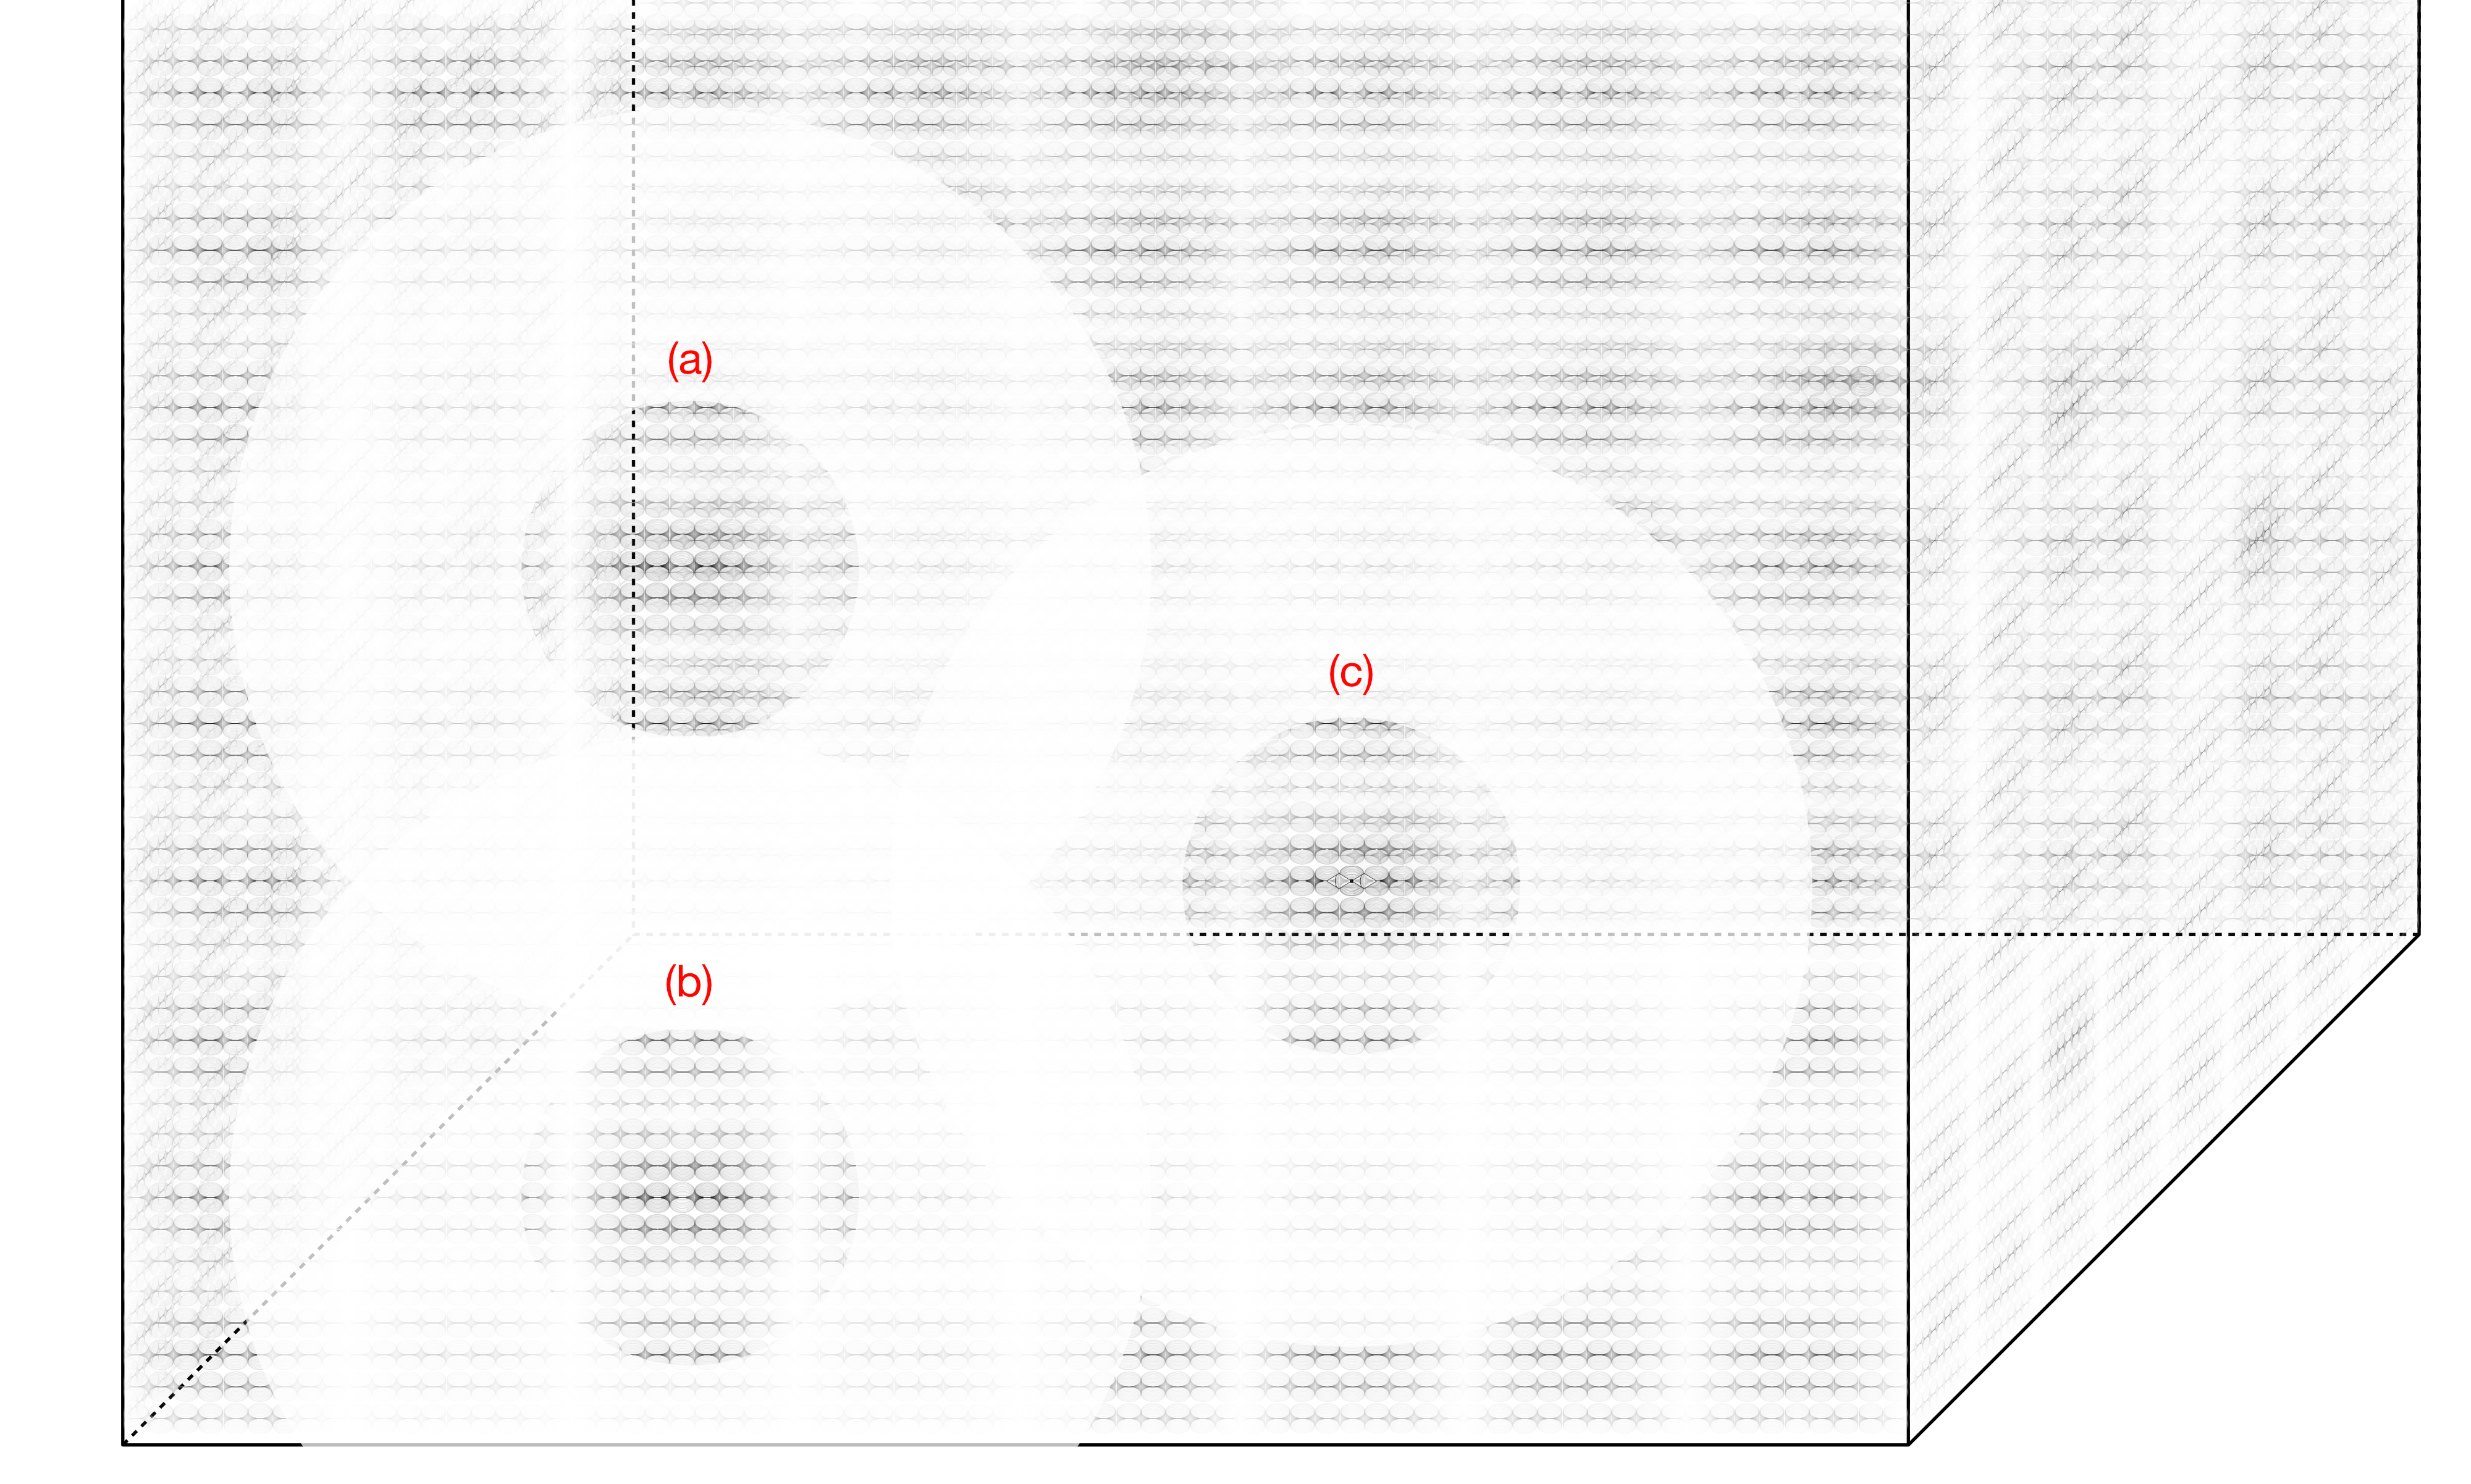
\includegraphics[width=0.8\linewidth]{figures/4.5.png}
    \caption[Larger field of horn tori as point plot heatmap]{\textbf{ Larger field of horn tori as point plot heatmap.}}
    \label{f4.5}
\end{figure}
\FloatBarrier


\section{Experiment to test computational information management of a hyperlinked research database}

\begin{figure}[h]
    \centering
    \includegraphics[width=\linewidth]{figures/4.6.png}
    \caption[Obsidian network graph of my research database and detail]{\textbf{Obsidian network graph of my research database and detail.}}
    \label{f4.6}
\end{figure}
\index[terms]{network graph}

To test the production of network graphs in PKM, I began my work with Obsidian, a markdown language platform that allows users to hyperlink across text files \citep{obsidian_obsidian_nodate}. Obsidian user databases are called vaults, individual text files are called pages, bulleted lines of text are called blocks, and hyperlinks are called links. Users of Obsidian’s predecessor Roam Research \citep{roam_research_roam_nodate} or other similar platforms like Logseq \citep{logseq_logseq-_nodate} may be familiar with some of the terminology and Markdown language formatting \citep{gruber_markdown_2004} \citep{swartz_html2text_2011}. 
\index[people]{Swartz, Aaron}
\index[people]{Gruber, John}

I set up my workflow for collecting sources and linking them following courses by Danny Hatcher \citep{hatcher_become_nodate}) and Lisa-Marie Cabrelli \citep{cabrelli_roam_nodate}. I consulted with Jay L. Colbert \citep{colbert_about_2022} to set up synchronization of my Obsidian and Logseq databases. 

As part of my survey of similar platforms I tested Logseq which had an attractive default mode for outlining text using collapsable lists of nested bullet points. I built an index of the names of every page generated in my Logseq database by creating an alphabetized list of page names in an automatically updating list. I modified the string query code by Logseq discussion forum user starryvechsh \citep{noauthor_how_2022} and created a page with queries for pages with names beginning with each letter of the alphabet, for pages beginning with each arabic numeral, and for pages beginning with any of Adler's syntopical terms. For example, this is my Markdown code for the letter `a':
\begin{verbatim}
#+BEGIN_QUERY
{
  :title "Pages that start with a"
  :query [
    :find (pull ?p [*])
    :where [
      [?p :block/name ?name]
      [(clojure.string/starts-with? ?name "a")]
    ]
  ]
}
#+END_QUERY
\end{verbatim}
\index[people]{Adler, Mortimer J.}


Logseq’s convenient collapsible lists of bullet points allowed me to create a page that indexes all blocks in my database that start with any given letter. I also added a section to query for any string of characters starting with a given number. As an exercise in information categorization and to expand on Adler’s Syntopicon\citep{adler_great_1952-2}, I also created an index using Adler’s 102 Great Ideas. The full version of the above code is available in \href{https://github.com/orusmateo/Orus-MCS-Thesis}{my GitHub Repository for this thesis}, and also listed in Appendix A.2. 
\index[people]{Adler, Mortimer J.}

\section{Experiment to test topic modeling between semantic fields for interdisciplinary knowledge translation}
As a person raised Roman Catholic working towards climate crisis mitigation, I made topic models to better understand the relationships between the papal encyclical \textit{Laudato si’} \citep{bergoglio_laudato_2015} and the \textit{Synthesis Report of the IPCC Sixth Assessment Report} \citep{lee_ipcc_2023}. 
 
Using the platform InfraNodus \citep{paranyushkin_infranodus_2019,paranyushkin_infranodus_nodate-2}, I created a topic model that graphed the intersecting themes of these two influential documents from different semantic fields in pursuit of knowledge translation between them. The result included ten names for groups of high-level ideas among the intersected graph:  (1) development equity, (2) environmental justice, (3) climate emissions, (4) disaster risk, (5) community development, (6) religious ethics, (7) global emissions, (8) climate resilience, (9) climate action, and (10) sustainable energy. InfraNodus notes in a tool-tip within the interface that its High-Level Ideas were generated using GPT-4.
\index[people]{Paranyushkin, Dmitry}
\index[terms]{InfraNodus}
\FloatBarrier
\begin{figure}[h]
    \centering
    \includegraphics[width=0.6\linewidth]{figures/4.8.png}
    \caption[InfraNodus graph of intersecting themes in \textit{Laudato si'}]{\textbf{InfraNodus graph of intersecting themes in \textit{Laudato si'} and the \textit{Synthesis Report of the IPCC Sixth Assessment Report}}. Ten high-level ideas are identified here by InfraNodus and labeled in bright colours as (1) development equity, (2) environmental justice, (3) climate emissions, (4) disaster risk, (5) community development, (6) religious ethics, (7) global emissions, (8) climate resilience, (9) climate action, and (10) sustainable energy. Used with permission.}
    \label{fig:4.8}
\end{figure}
\FloatBarrier
\par
I found that there are concepts present in the \textit{Synthesis Report of the IPCC Sixth Assessment Report} but missing in \textit{Laudato si'}, and vice versa. I was concerned to find that ‘adaptation’ and ‘mitigation’ were not a part of \textit{Laudato si’}. Conversely, the \textit{Synthesis Report of the IPCC Sixth Assessment Report} did not include the terms `god’ and `church’ which is unsurprising considering it is not a theological document.

InfraNodus also provided a list of entry points to develop each text, what it calls conceptual gateways. In addition to the previous missing concepts to develop \textit{Laudato si’} this topic model recommended developing the ideas of `infrastructure’ and `warming’. 
\index[terms]{InfraNodus}

\FloatBarrier
\begin{figure}[h]
    \centering
    \includegraphics[width=0.8\linewidth]{figures/4.9.png}
    \caption[Missing Concepts listed within the Blind Spots tab in the Text Analytics Panels of InfraNodus]{ Missing Concepts listed within the Blind Spots tab in the Text Analytics Panels of InfraNodus. Comparison of missing concepts: (left) concepts in the Synthesis Report of the \textit{IPCC Sixth Assessment Report} but missing from \textit{Laudato si'}; (right) concepts in \textit{Laudato si'} but missing from the Synthesis Report of the \textit{IPCC Sixth Assessment Report}. Used with permission.}
    \label{fig:4.9}
\end{figure}
\index[terms]{InfraNodus}

\begin{figure}[h]
    \centering
    \includegraphics[width=0.8\linewidth]{figures/4.10.png}
    \caption[Conceptual Gateways listed within the Blind Spots tab in the Text Analytics Panels of InfraNodus]{Conceptual Gateways listed within the Blind Spots tab in the Text Analytics Panels of InfraNodus.  Comparison of conceptual gateways as ``ideas to extend this discourse": (left) gateways for \textit{Laudato si'}; (right) gateways for the \textit{Synthesis Report of the IPCC Sixth Assessment Report}. Used with permission.
}
    \label{fig:4.10}
\end{figure}
\FloatBarrier
\index[terms]{InfraNodus}


\section{Experiment to test more ecological local AI}
\begin{quote}
    ``\textit{The ecology of the vast symbolic world has to be supported by a material infrastructure of sustainability and responsibility, and turning our back on the real is no way to guarantee the virtual}” \citep[p. 196]{drucker_graphesis_2014}. 
\end{quote}
Since my thesis works to apply the ``studio laboratory of knowledge design” \citep[p. 197]{drucker_graphesis_2014}  and ``knowledge engineering” \citep[p. 8]{wielinga_kads_1992}  behind Sustainability Transitions Knowledge Activation, it is foundational to approach this work while managing its ecological cost. AI, in particular, has a large and growing cost that is ``widening disparity in how different regions and communities are affected” \citep{ren_uneven_2024}. 
\index[terms]{Sustainability Transitions} \index[terms]{Knowledge Activation (KA)} \index[terms]{Sustainability Transitions Knowledge Activation (STKA)} 
\index[people]{Drucker, Johanna}

Considering environmental costs of using AI, I moved to test topic modeling using small language models that can run on my local workstation. Computer scientist Rahul Nayak proposes one such solution to create what he refers to as graphs of concepts using Mistral 7B, named after its comparably small seven billion parameters \citep{nayak_how_2023}.

Software engineer Juan Sulca and I successfully used Nayak’s method to create a navigable and searchable graph of concepts of \textit{Laudato si’}. However, further development would be required to create a comparison graph such as the one generated by InfraNodus.
\index[terms]{InfraNodus}

\begin{figure}[h]
    \centering
    \begin{minipage}[t]{0.48\linewidth}
        \centering
        \includegraphics[width=\linewidth]{figures/4.11.png}
        \caption[Overview of the \textit{Laudato si'} graph of concepts]{Overview of the \textit{Laudato si'} graph of concepts made using Rahul Nayak’s Mistral 7B method.}
        \label{f4.11}
    \end{minipage}%
    \hfill
    \begin{minipage}[t]{0.48\linewidth}
        \centering
        \includegraphics[width=\linewidth]{figures/4.12.png}
        \caption[Detailed view of the \textit{Laudato si'} graph of concepts]{Detailed view of the \textit{Laudato si'} graph of concepts made using Rahul Nayak’s Mistral 7B method.}
        \label{f4.12}
    \end{minipage}
\end{figure}

\par
Facing the limit of my ability to produce three-dimensional topic models on a local LLM, I turned to making moving spatial network graphs to examine them in relation to other forms of information visualization. 
\index[terms]{Large Language Model (LLM)}


\section{Observations about information practices in the University}
A number of political and economic factors actively detract from climate mitigation. For example, hyper-specialization is convenient for the current predominantly empire-driven capitalist extractivist economy; hyper-specialization makes humans monocrops for convenient harvesting through overwork, which keeps large populations politically docile consumers. It seems to me that it is convenient to keep researchers underinformed about solutions from other fields that support climate mitigation because this means those solutions can be bought and sold. Specialization is required to achieve proficiency in order to make an impact in any field, but isolation-reinforced hyper-specialization does not have to be the norm.
\index[terms]{network graph}

As the earth careens toward catastrophe, resistance will inevitably ensue, and it will be the prerogative of political oppressors to control populations by predictably harsher means like conscription to armed conflict. It is in the imperfect container of the University that people have historically had, and still may have, some leverage to resist the ideological and technological limitations to better climate mitigation. 

In the experience of discussing my research, I have observed that many organizations, including universities, struggle with how to best use available information to facilitate researcher grouping, which significantly affects which funding a given group can access. The struggle for connecting researchers only heightens my urgency to build better tools for connecting ideas, and the people who have them, to reveal solutions for climate crisis mitigation that may exist in the information we already have. 

It is at this point that I begin the bulk of research that underlies my contributions to the space of graph-making and analysis.
